\section{Проектирование программного средства}
\label{sec:arch}

\section{Архитектура ПС}
\label{sec:arch_arch}

При проектировании архитектуры програмного средства я иходил из следующих побуждений:
\begin{itemize}
	\item обработка изображений требует хорошей производительности компьютера;
	\item у оператора должна быть возможность управлять процессом пропуска;
	\item програмное средство должно быть легко расширяемо с точки зрения изменения оработчика результатов распознанного номера;
	\item процесс обработки изображения представляет из себя последовательное выполенения сложных операций;
\end{itemize}

Для предоставления программе хороших вычислительных мощностей можно поместить её на мощьных сервер а клиенту лишь посылать результаты выполенения. Напрашивается вывод что для приложения лучше использовать клиент-серверную архитектуру. 

\begin{figure}[ht] 
    \centering
    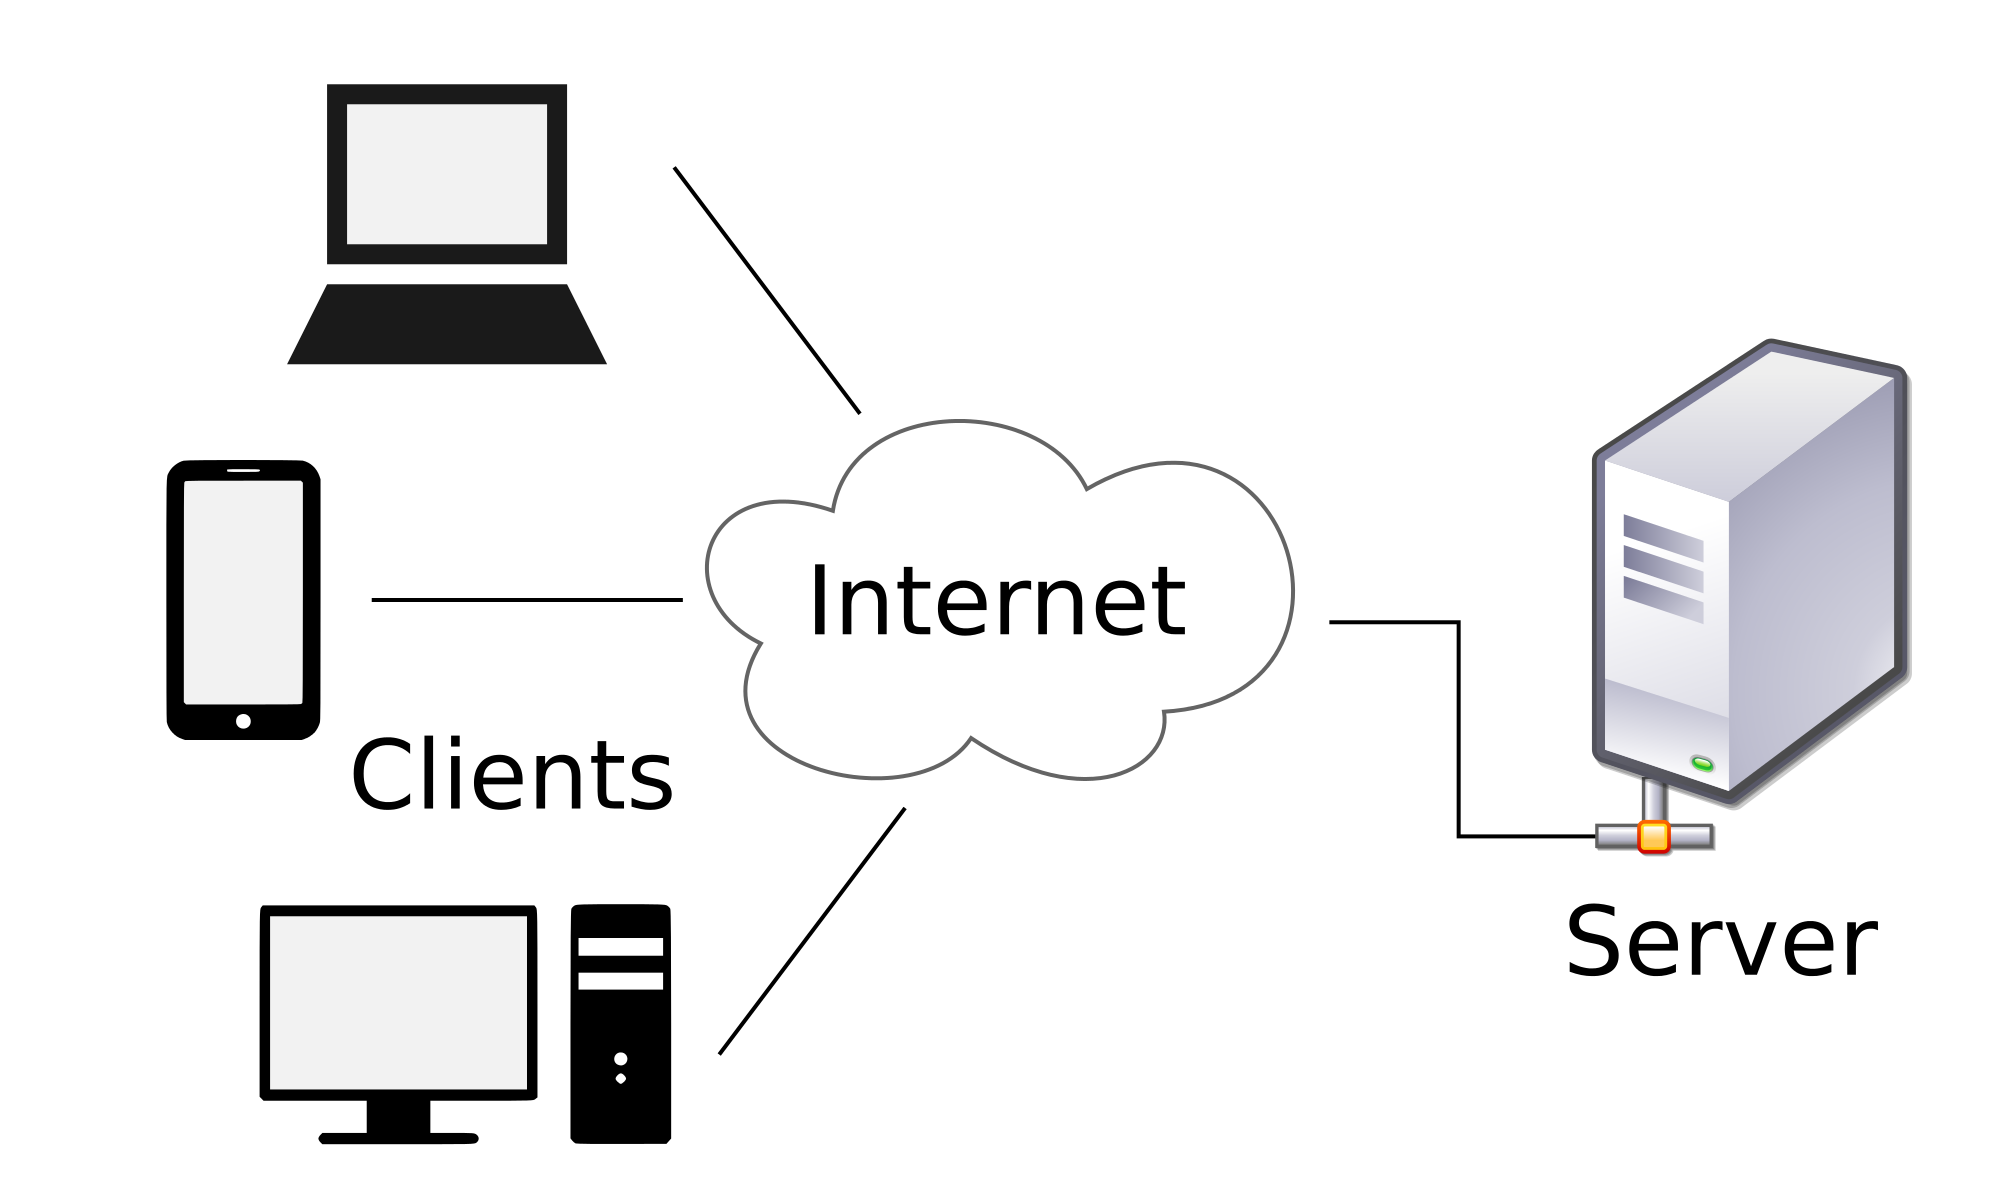
\includegraphics[scale=0.2]{Client-server-model.png}  
    \caption{Наглядная схема работы клиент-серверного приложения}
    \label{fig:arch_arch:client_server}
\end{figure}

Клиент-сервер - вычислительная или сетевая архитектура, в которой задания или сетевая нагрузка распределены между поставщиками услуг, называемыми серверами, и заказчиками услуг, называемыми клиентами. Физически клиент и сервер — это программное обеспечение. Обычно они взаимодействуют через компьютерную сеть посредством сетевых протоколов и находятся на разных вычислительных машинах, но могут выполняться также и на одной машине. Программы - сервера, ожидают от клиентских программ запросы и предоставляют им свои ресурсы в виде данных

Так же клиентскую часть лучше всего реализовать с помощью технологий html/css/java script. Это позволит использовать приложения практически с любого клиенского оборудование включая планшеты, компьютеры и телефоны. Общую схему работы приложения можно увидеть на рисунке \ref{fig:arch_arch:client_server}

Процесс обработки изображений представляет из себя последовательно применение различных алгоритмов для исходного изображения. Конкретно эту часть лучше всего сделать используя архитектуру "Каналы и фильтры". Этот вид архитектуры подходит в том случае, если процесс работы приложения распадается на несколько шагов, которые могут выполнятся отдельными обработчиками. Основными компонентами являются "фильтр" и "канал". Иногда дополнительно выделяют "источник данных" и "потребитель данных". Приминительно к разрабатыемому програмному продукту, фильтр это конкретный алгоритм обрабатывающи изображение, источник данных - это видео поток от IP камеры, потребителем данных будут явятся плагины.

\begin{figure}[ht] 
    \centering
    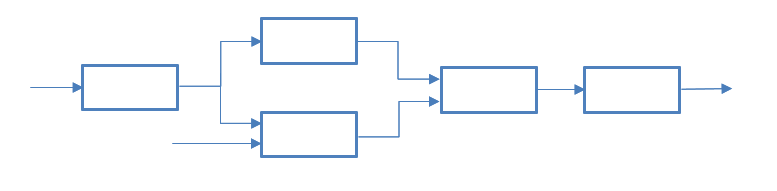
\includegraphics[scale=0.8]{pipes_and_filters.png}  
    \caption{Каналы и фильтры}
    \label{fig:arch_arch:pipes_and_filters}
\end{figure}

Каждый поток обработки данных – это серия чередующихся фильтров и каналов, начинающаяся источником данных и заканчивающаяся их потребителем. Каналы обеспечивают передачу данных и синхронизацию. Фильтр же принимает на вход данные и обрабатывает их, трансформируя в некое иное представление, а затем передает дальше.

Архитектура фильтров позволяет добится хорошо читаемого кода потому как реализует один из самых сложных принципов SOLID: принцип единственной обязанности, заключающийся в том что класс должен иметь только одну ответственность, то есть повлиять на спецификацию класса должно быть способно только одно потенциальное изменение в спецификации ПО. 